\documentclass[11pt]{beamer}

\usepackage[utf8]{inputenc}
\usepackage[spanish]{babel}
\usepackage{hyperref}

\title{Sistemas Embebidos con el ARM-Cortex-M4}
\subtitle{Introducción a la Arquitectura ARM}
\author[AK]{Alejandro S. Kelly}
\institute[]{Pulsar Labs}


\begin{document}

    \frame{\titlepage}

    \section{Introducción}

        \begin{frame}
            \frametitle{¿Por que ARM-Cortex?}

            Los procesadores ARM se caracterizan por alto desempeño a bajo costo y potencia. \hfill\break\break 
            Combinan capacidades de procesamiento digital de señales, control, y computación de propósito general en una arquitectura facil de programar y depurar. \hfill\break\break 
            Además, hay más de 230 miles de millones de unidades en el mundo. 
        \end{frame}

        \begin{frame}
            \frametitle{La familia Cortex}

            La familia Cortex se divide en 3 tipos principales, A, R y M. Todos son una variante de Armv\{6,7,8\}, pero optimizados para aplicaciones móviles y/o embebidas.
            La clasificacion es la siguiente: 
                
            \begin{description}
                \item[A] Procesadores de Aplicacion. 
                \item[R] Procesadores para seguridad funcional.
                \item[M] Procesadores para microcontroladores de propósito general. 
            \end{description}
        \end{frame}

        \begin{frame}
            \frametitle{Cortex-M}

            La familia Cortex-M también tiene su \href{run:./Resources/CORTEX_COMPARISON.pdf}{clasificacion interna}:
            
            \begin{description}
                \item[M0] El rango de entrada de la familia, menores velocidades y menos soporte de instrucciones y depuración. 
                \item[M1] Cortex sintetizable, para FPGA's.
                \item[M3] Núcleos potentes para microcontroladores más pequeños.
                \item[M4] DSP y FPU incluidos, mejor depuración y velocidad, son los procesadores más populares.
                \item[M7] DSP y FPU avanzados, soporte de coprocesadores, cache de instrucciones, buses avanzados.
            \end{description}
        \end{frame}

        \begin{frame}
            \frametitle{¿Por que el CM4?}

            Es un excelente punto de partida, ya sea a mayores o menores capacidades. 
            
            Además, hay una oferta muy variada por parte de los fabricantes, especialmente de STMicroelectronics, por ello, utilizaremos un Kit de desarrollo STM32F4Discovery. 

        \end{frame}

    \section{Review de Arquitectura}

        \begin{frame}
            \frametitle{El modelo de procesador.}

            \begin{center}
                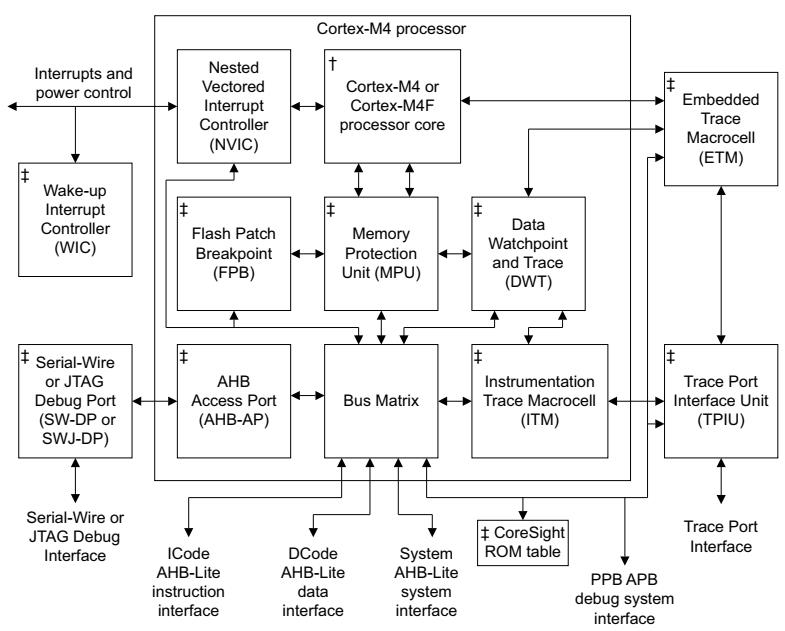
\includegraphics[scale = 0.4]{./Resources/CM4_MODEL.jpg}
            \end{center}
        \end{frame}

        \begin{frame}
            \frametitle{NVIC}

            El Nested Vector Interrupt Controller (NVIC) es un elemento esencial de la arquitectura ARM.
            
            Es un controlador y enrutador de interrupciones (excepciones)

        \end{frame}

\end{document}
